% Draft. Every decimal number in sections/*.tex must trace to paper/numbers.json
% (python analysis/paper_numbers.py, then python analysis/check_paper_numbers.py).
% Style: no em dashes; formulas in LaTeX.
\documentclass[11pt]{article}
\usepackage[margin=1in]{geometry}
\usepackage{amsmath,amssymb}
\usepackage{booktabs}
\usepackage{graphicx}
\usepackage[numbers]{natbib}
\usepackage[hidelinks]{hyperref}
\graphicspath{{../para_figures/}}

\newcommand{\eg}{e.g.,\ }
\newcommand{\ie}{i.e.,\ }

\title{Does the Support Set Steer the Step?\\An Analysis of Prompt-Anchored Residual Adaptation\\for Biomedical Vision-Language Models}
\author{Draft}
\date{\today}

\begin{document}
\maketitle

\begin{abstract}
Few-shot adaptation of biomedical vision-language models depends on which examples are drawn.
Prompt-Anchored Residual Adaptation (PARA) addresses this by keeping the frozen prompt prediction as an anchor
and moving towards a prediction trained on the support set by a step computed from the geometry of the support embeddings.
We reimplement PARA on BiomedCLIP and study the step on six MedMNIST datasets, three used for design and three held out,
with repeated support draws, balanced accuracy and worst-case (CVaR20) evaluation.
We find that the geometric signals barely depend on the class in BiomedCLIP's frozen space,
so the step reduces to the same function of the number of shots on every dataset ($0.33$, $0.60$ and $0.80$ at 1, 4 and 16 shots),
predictable from two constants of the pretrained model; a schedule in the shot count alone does better.
On binary tasks, standardizing each branch's scores turns the blend into a switch: PARA returns the zero-shot prediction below a step of $0.5$
and the trained branch's prediction above it, on every image.
The best step instead follows how reliable the anchor is relative to the trained branch;
a rule based on the anchor's reliability alone, fixed before the held-out runs, improved on the design datasets and failed on the held-out ones.
Blending log-probabilities instead of standardized scores, with no new parameters, raises balanced accuracy by $4.86$ points on multi-class datasets
but lowers the worst case where the anchor is good.
We conclude with recommendations for evaluating adaptive blending: check that adaptive signals vary across support draws,
compare against shot-only and single-branch baselines, include binary tasks, and test on held-out data.
\end{abstract}


\section{Introduction}\label{sec:intro}

Biomedical vision-language models such as BiomedCLIP \citep{zhang2023biomedclip} classify images zero-shot from text prompts,
and a few labelled examples per class can adapt them further \citep{koleilat2025biomedcoop}.
With so few examples, however, the adapted model depends on which examples were drawn.
A support set that happens to be unrepresentative can produce a classifier much worse than the zero-shot one,
and in medical use the worst plausible outcome matters at least as much as the average.

Prompt-Anchored Residual Adaptation (PARA) \citep{kang2026para} addresses this directly.
It keeps the frozen prompt prediction as an anchor that no support set can change,
learns a visual prediction from the support set, and moves from the anchor towards it by a residual step $\eta(S)$.
The step is computed in closed form from the frozen support embeddings, from how far the class images lie from their text and how consistently they agree,
so that a support set which disagrees with the prompts earns a larger step.
PARA also introduces a repeated-support protocol that reports the worst $20\%$ of support draws (CVaR20) alongside the mean,
and reports state-of-the-art results on both.

This paper asks whether the support set actually steers PARA's step, and what happens when it does not.
We reimplement PARA on BiomedCLIP and study it on six MedMNIST datasets with its own repeated-support protocol, balanced accuracy and CVaR20.
Three datasets were used to develop every analysis; three others were chosen afterwards and serve as held-out tests,
including a rule whose constant was fixed before any held-out model was trained.
Our findings are:
\begin{enumerate}
  \item \textbf{The step is a fixed curve in the number of shots} (Section~\ref{sec:finding1}).
  In BiomedCLIP's frozen space, the discrepancy and agreement signals barely depend on the class:
  images sit about equally far from every class's text, and any set of images agrees almost as much as a real class.
  The step is therefore the same function of $K$ on every dataset ($0.33$, $0.60$ and $0.80$ at $K = 1$, $4$ and $16$),
  predictable from two constants of the pretrained model.
  A schedule that uses $K$ alone does better than PARA's step (significantly in 13 of 18 design settings, never worse).
  \item \textbf{On binary tasks the blend is a switch} (Section~\ref{sec:finding2}).
  Standardizing each branch's scores across two classes keeps only the sign of the prediction,
  so PARA returns the zero-shot prediction whenever $\eta < 0.5$ and the trained branch's prediction whenever $\eta > 0.5$, on every image.
  We prove this and confirm it on all 1,046 relevant evaluations.
  \item \textbf{The right step depends on the anchor's reliability relative to the trained branch} (Section~\ref{sec:finding3}).
  The best step in hindsight ranges from $0.17$ to $0.95$ across datasets and shot counts, and follows how good the anchor is compared with the trained branch.
  A rule based on the anchor's reliability alone, fixed in advance, improved on the design datasets and failed on the held-out ones.
  \item \textbf{Blending log-probabilities helps on multi-class tasks} (Section~\ref{sec:finding4}).
  With the same step and the same trained models, blending each branch's log-probabilities instead of its standardized scores
  raises mean balanced accuracy by $4.86$ points on multi-class datasets, but lowers the worst case where the anchor is good.
\end{enumerate}
From these we draw practical recommendations for evaluating adaptive blending (Section~\ref{sec:discussion}).
We do not claim that PARA is worse than other few-shot methods, and we do not reproduce its benchmark numbers;
our subject is how its step behaves and what a step of this kind would need to do.
% TODO: code and prompt-mapping release statement, once decided.

\section{Related work}\label{sec:related}

\paragraph{Few-shot adaptation of vision-language models.}
Contrastive vision-language models such as CLIP \citep{radford2021clip} are adapted to new tasks with a few labelled examples in two broad ways.
Prompt learning replaces hand-written prompts with learned context vectors \citep{zhou2022coop}.
Adapter and residual methods instead keep the pretrained prediction and add a learned correction:
CLIP-Adapter blends adapted and original features through a residual connection \citep{gao2024clipadapter},
Tip-Adapter adds a cache built from the support set to CLIP's zero-shot logits \citep{zhang2022tipadapter},
and TaskRes learns a residual on top of the frozen text classifier \citep{yu2023taskres}.
All of these combine a pretrained and a learned component, and the weight given to each is usually a hyperparameter.
In biomedical imaging, BiomedCLIP \citep{zhang2023biomedclip} provides the pretrained model,
and BiomedCoOp \citep{koleilat2025biomedcoop} and vMFCoOp \citep{shao2026vmfcoop} adapt prompt learning to it;
BiomedCoOp's GPT-4 class descriptions are also the prompts PARA uses.

\paragraph{Setting the blending weight without validation data.}
With a few examples per class there is rarely data to spare for validation, so several methods set the balance between pretrained and learned components without it.
ProLIP fine-tunes only CLIP's image projection, regularized towards its pretrained value,
and in its validation-free variant scales the regularization weight as $1/N$ in the number of shots per class \citep{fahes2026prolip}.
HOSO-Adapter holds out one support example per class to learn the blending ratio of CLIP-Adapter \citep{vorster2026hoso}.
PARA \citep{kang2026para} computes its step in closed form from the geometry of the frozen support embeddings, with no training and no held-out data.
Our shot-only and HOSO-style baselines follow the first two ideas, applied to PARA's blend, so that the three ways of setting the step can be compared on the same trained models.

\paragraph{Geometry of contrastive embedding spaces.}
\citet{liang2022mind} showed that CLIP-style models place image and text embeddings in separate regions of the shared space (the modality gap),
with each modality confined to a narrow cone.
These two properties explain our first finding: PARA's discrepancy mostly measures the gap, which is the same for every class,
and its agreement mostly measures the cone, which is the same for any set of images.
We build on their analysis rather than claim the phenomenon as new.

\paragraph{Evaluation under support-set variation.}
Because few-shot results depend on the sampled support set, PARA evaluates over repeated support draws and reports the worst $20\%$ as well as the mean.
We adopt this protocol, share the draws across every method so that comparisons are paired,
and add balanced accuracy, tests per setting with multiple-comparison correction, and a split into design and held-out datasets.

\section{Setup}\label{sec:setup}

\paragraph{PARA in brief.}
PARA \citep{kang2026para} combines two predictors for an image $x$ and classes $c = 1, \dots, C$.
The \emph{anchor} is the frozen zero-shot prediction
$z^0_c(x) = \tau_0 \langle F^0_v(x), t_c \rangle$, where $F^0_v$ is the frozen image encoder,
$t_c$ is the normalized mean embedding of an ensemble of class prompts, and $\tau_0$ is the frozen pretrained logit scale.
The \emph{support branch} is trained on the labelled support set $S$:
$z^S_c(x) = \tau_v \langle F^S_v(x), p^S_c \rangle$, with a LoRA-adapted encoder $F^S_v$ \citep{hu2022lora},
class prototypes $p^S_c$ and a learned scale $\tau_v$, trained with a leave-one-out prototype loss.
Each branch is standardized across classes (written $\bar z$), and the prediction moves from the anchor towards the support branch by a step $\eta(S)$:
\begin{equation}
  \hat z_c(x) = \bar z^0_c(x) + \eta(S)\,\big(\bar z^S_c(x) - \bar z^0_c(x)\big).
  \label{eq:blend}
\end{equation}
The step is computed in closed form from the frozen support embeddings $u_i = F^0_v(x_i)$, which, like $t_c$, are L2-normalized.
With $S_c$ the $n_c$ support images of class $c$, $h_c = \sum_{i \in S_c} u_i$ and $d_c = h_c / \lVert h_c \rVert$,
\begin{equation}
  \eta(S) = \frac{\lambda}{C} \sum_{c=1}^{C} \frac{\delta_c \phi_c}{1 + \delta_c \phi_c},
  \qquad
  \delta_c = 1 - \langle d_c, t_c \rangle,
  \qquad
  \phi_c = \frac{\lVert h_c \rVert^2}{n_c}.
  \label{eq:eta}
\end{equation}
The \emph{anchor discrepancy} $\delta_c$ is meant to measure how far the class images lie from their own text,
and the \emph{support agreement} $\phi_c$ how consistently they point the same way.
$\lambda = 0.9$ on every dataset.

\paragraph{Reimplementation.}
No official code has been released, so we reimplemented PARA from the paper.
The backbone is BiomedCLIP ViT-B/16 \citep{zhang2023biomedclip}, with $\tau_0 = 85.23$.
LoRA uses rank $8$ and $\alpha = 16$ on the image encoder.
Following the paper, we train for $80$ epochs with AdamW (learning rate $10^{-4}$ for LoRA and $10^{-3}$ for $\tau_v$, weight decay $10^{-4}$)
and keep the final checkpoint.
Two details the paper leaves open we set ourselves: a batch size of $32$ and random resized crops with scale $(0.5, 1)$ plus horizontal flips.
As a check, BiomedCoOp's GPT-4 prompts give a DermaMNIST zero-shot accuracy of $53.55\%$ in our implementation,
against $53.78\%$ for zero-shot BiomedCLIP in Table A3 of \citet{kang2026para}.
This confirms that the pipeline matches theirs, not that the anchor is useful: both are below the $66.7\%$ obtained by always predicting
the majority class (nevi), and the corresponding BAcc is $21.39\%$ (Table~\ref{tab:T1_datasets}).

\paragraph{Datasets and prompts.}
We use six 2D datasets from MedMNIST v2 \citep{yang2023medmnist} (Table~\ref{tab:T1_datasets}):
DermaMNIST at $224$ pixels and the other five at $128$ pixels (all resized to the encoder's $224$-pixel input).
Each dataset is scored on a fixed test subset.
Because splits and resolution differ from the paper's benchmark, our absolute numbers are not directly comparable to it.
Every dataset uses our own prompt ensemble:
five hand-written visual descriptions per class for DermaMNIST, and five generic templates for the other datasets.
Where BiomedCoOp \citep{koleilat2025biomedcoop} provides GPT-4 descriptions for exactly matching classes,
we add them as a second prompt set (50 per class): DermaMNIST, OCTMNIST and BloodMNIST,
and BreastMNIST via its source dataset BUSI, with BUSI's ``benign'' and ``normal'' descriptions pooled into MedMNIST's merged class.

\begin{table}[t]
\centering
\small
\caption{Datasets. Zero-shot BAcc (\%) on the evaluated test subset, per prompt set. ``Your prompts'' are 5 hand-written visual descriptions per class for DermaMNIST and 5 generic templates elsewhere; GPT-4 prompts are BiomedCoOp's (BreastMNIST via BUSI: benign and normal pooled). ZS: zero-shot.}
\label{tab:T1_datasets}
\begin{adjustbox}{max width=\linewidth}
\begin{tabular}{lrrrrrl}
\toprule
Dataset & Classes & Test images & Pixels & ZS BAcc, own & ZS BAcc, GPT-4 & Split \\
\midrule
DermaMNIST & 7 & 2000 & 224 & 20.93 & 21.39 & design \\
OCTMNIST & 4 & 1000 & 128 & 49.30 & 51.50 & design \\
BloodMNIST & 8 & 2000 & 128 & 14.86 & 13.49 & design \\
BreastMNIST & 2 & 156 & 128 & 53.63 & 70.93 & held-out \\
PneumoniaMNIST & 2 & 624 & 128 & 67.35 & -- & held-out \\
OrganAMNIST & 11 & 2000 & 128 & 25.71 & -- & held-out \\
\bottomrule
\end{tabular}
\end{adjustbox}
\end{table}


\paragraph{Protocol.}
For each dataset we use $K \in \{1, 4, 16\}$ shots per class and draw 10 support sets per $K$.
The draws are made once and shared by every step rule and both prompt sets, and the support branch is trained once per draw
(one training seed) and cached.
Every step rule below is therefore applied to identical trained models, and differences between rules are paired by draw.
Our primary metric is balanced accuracy (BAcc), because plain accuracy rewards majority-class predictions
(on DermaMNIST, about two thirds of test images are nevi).
We also report CVaR20, the mean BAcc over the worst $20\%$ of draws (the worst 2 of 10), which is PARA's own worst-case measure,
and Macro-F1.
For paired comparisons we run a Wilcoxon signed-rank test over the 10 draws of each setting (dataset, prompt set, $K$),
count settings significantly better or worse at $p < 0.05$, and also report counts after Holm's correction within each family of settings.
With 10 draws the smallest attainable two-sided $p$ is $2/1024 \approx 0.002$, so Holm-significant settings are those
in which nearly every draw moves in the same direction.

\paragraph{Step rules compared.}
Besides PARA's $\eta(S)$ we evaluate, on the same trained models:
zero-shot ($\eta = 0$); visual only ($\eta = 1$);
a \emph{shot-only} schedule $\eta_K = \lambda K / (1 + K)$, which uses the shot count and nothing else
(shot-dependent schedules are prior art, \eg ProLIP \citep{fahes2026prolip}, so we treat it as a baseline);
a HOSO-style step chosen on one held-out shot per class \citep{vorster2026hoso};
and an oracle that picks the best $\eta$ on the test set for each draw, reported only as an upper bound.

\paragraph{Design and held-out datasets.}
DermaMNIST, OCTMNIST and BloodMNIST were used to develop every analysis and rule (\emph{design} datasets).
PneumoniaMNIST, BreastMNIST and OrganAMNIST were chosen afterwards from a zero-shot screening alone,
before any model was trained on them, and serve as \emph{held-out} datasets.
The one tuned rule in this paper, the anchor-aware step of Section~\ref{sec:finding3},
has a single constant $c$. We fixed $c = 8$ because it maximized CVaR20 BAcc pooled over the three design datasets
($56.07$, against $55.71$ for $c = 4$ and $55.61$ for $c = 16$); this choice is in-sample on those datasets.
We made this choice between the last design analysis and the first held-out training run, but the evidence for that timing is weak.
The decision itself was not recorded with a date: the held-out runs scored all nine values of $c$ without marking one as chosen,
and the first committed record of $c = 8$ postdates the held-out runs.
The zero-shot screening, which also computed $r_a$ on the held-out candidates, may have preceded the choice.
We therefore call it a pre-specified rule, not a registered one; that $c = 8$ is not the best value on the held-out data
(Section~\ref{sec:finding3}) argues against a choice informed by held-out results, but does not prove the order.

\section{The support geometry is uninformative, so the step is a fixed curve in $K$}\label{sec:finding1}

PARA's step is meant to adapt to the support set: a support set that disagrees with the text should earn a larger step.
On all six datasets, however, $\eta(S)$ is almost entirely determined by the number of shots.
Pooled over datasets and prompt sets, its mean is $0.328$, $0.603$ and $0.798$ at $K = 1$, $4$ and $16$ (Figure~\ref{fig:eta_vs_K}).
The per-dataset means span only $0.316$ to $0.353$, $0.587$ to $0.610$ and $0.790$ to $0.802$,
even though the datasets range from 2 to 11 classes and from near-chance to fairly strong zero-shot anchors.
Across the 10 support draws of a setting, the standard deviation of $\eta(S)$ never exceeds $0.011$.
This section explains why, and shows that a step depending on $K$ alone does at least as well.

\begin{figure}[t]
  \centering
  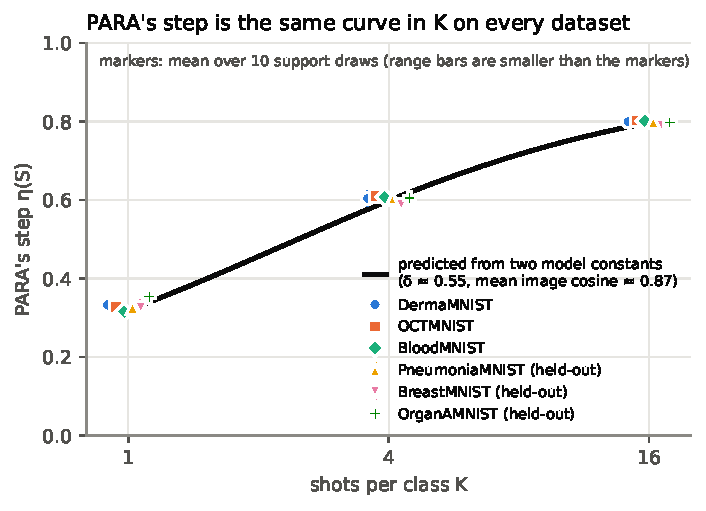
\includegraphics[width=0.62\linewidth]{F1_para_eta_vs_K}
  \caption{PARA's step $\eta(S)$ against shots per class, mean over 10 support draws for each dataset
  (draw-to-draw ranges are smaller than the markers).
  The curve is the prediction of Eq.~\eqref{eq:pred} from two constants of the frozen model,
  $\bar\delta = 0.550$ and the pooled image cosine $0.867$.}
  \label{fig:eta_vs_K}
\end{figure}

\paragraph{The discrepancy $\delta_c$ does not depend on the class.}
Figure~\ref{fig:geometry} (top left) compares, for $K = 16$ and one support draw, each class's discrepancy to its own text
with its discrepancy to the other classes' text.
On five datasets the two differ by only $0.004$ to $0.018$; OrganAMNIST shows the largest gap
($0.604$ against $0.647$).
The support images of a class are closest to their own class text for only one or two classes per dataset
(three of eleven on OrganAMNIST).
In BiomedCLIP's frozen space, image and text embeddings occupy separate regions, the modality gap described by \citet{liang2022mind},
so $\delta_c$ mostly measures the distance between the two modalities, which is the same for every class.
Averaged over the six datasets, the own-text discrepancy is $\bar\delta = 0.550$.

\paragraph{The agreement $\phi_c$ does not depend on the class either.}
Sixteen images of one class give almost the same $\phi_c$ as sixteen random images drawn across classes
(Figure~\ref{fig:geometry}, bottom left): the two differ by at most $1.3\%$ on five datasets and by $16\%$ on OrganAMNIST.
The reason is that the frozen image embeddings lie in a narrow cone.
The mean cosine between two support images is $0.839$ to $0.962$ on five datasets, whether or not the images share a class,
and $0.671$ for different-class pairs on OrganAMNIST.
Because the $u_i$ have unit length, $\phi_c$ is an exact function of that cosine:
\begin{equation}
  \phi_c = \frac{1}{n_c} \Big\lVert \sum_{i \in S_c} u_i \Big\rVert^2 = 1 + (n_c - 1)\,\bar c_c,
  \label{eq:phi}
\end{equation}
where $\bar c_c$ is the mean pairwise cosine within class $c$.
When every pair of images has a cosine near 0.9, $\phi_c$ is close to its maximum $n_c = K$ for any class, and for a random set of images as well.

\begin{figure}[t]
  \centering
  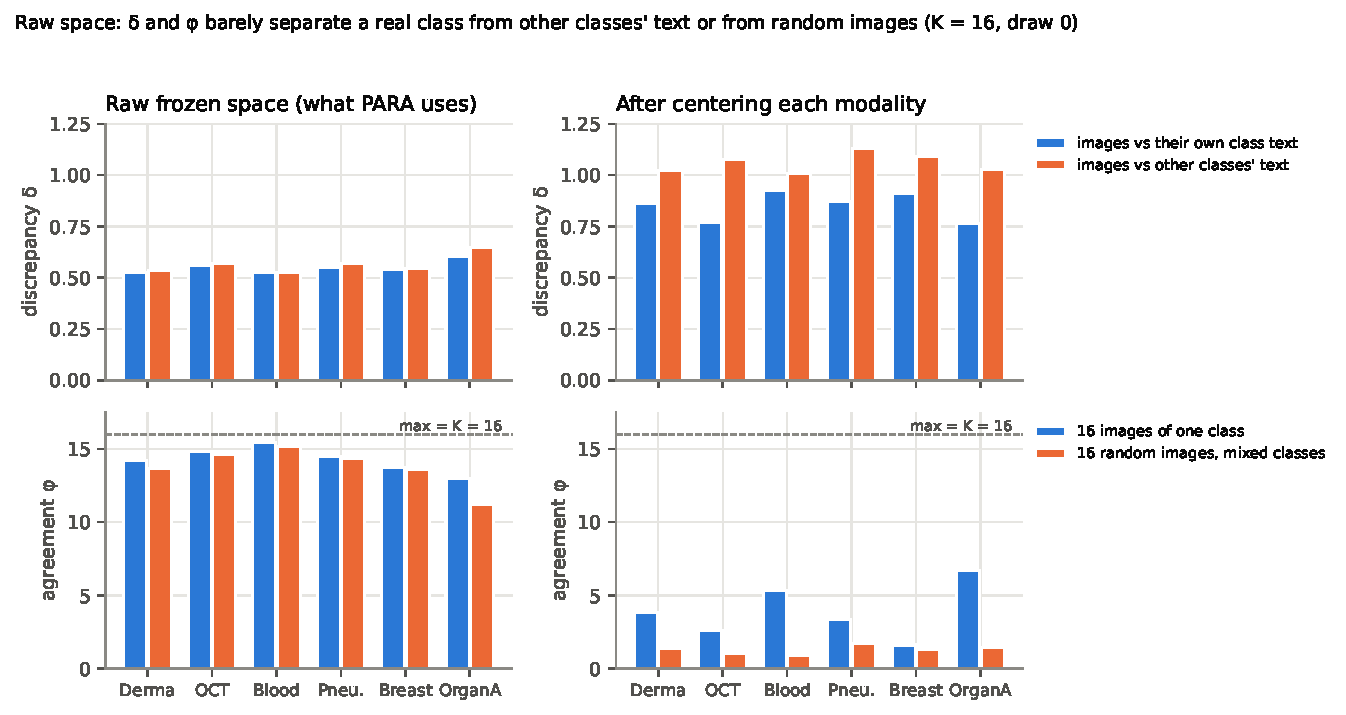
\includegraphics[width=\linewidth]{F2_geometry_check}
  \caption{Support geometry for $K = 16$, one draw per dataset.
  Top: discrepancy of each class's images to their own text and to the other classes' text.
  Bottom: agreement $\phi$ of 16 images of one class against 16 random images from mixed classes.
  Left: the raw frozen space that PARA uses. Right: after subtracting each modality's mean.}
  \label{fig:geometry}
\end{figure}

\paragraph{Two constants predict the step.}
If every class has $\delta_c \approx \bar\delta$ and $\bar c_c \approx \bar c$, Eqs.~\eqref{eq:eta} and~\eqref{eq:phi} give
\begin{equation}
  \eta(K) \approx \lambda\,\frac{a(K)}{1 + a(K)}, \qquad a(K) = \bar\delta\,\big(1 + (K - 1)\,\bar c\big).
  \label{eq:pred}
\end{equation}
With $\bar\delta = 0.550$ and the mean same-class cosine $\bar c = 0.886$, Eq.~\eqref{eq:pred} predicts
$0.319$, $0.601$ and $0.798$ at $K = 1$, $4$ and $16$, against the measured $0.328$, $0.603$ and $0.798$.
Using the cosine pooled over same- and different-class pairs ($0.867$, the curve in Figure~\ref{fig:eta_vs_K}) changes the prediction by about $0.003$ at most,
which is itself a symptom: the class structure that $\phi_c$ is meant to detect hardly registers.
At $K = 1$, $\phi_c = 1$ exactly, so the step there depends on $\delta_c$ alone.

OrganAMNIST deserves a note, because it is the one dataset where the geometry does carry some class signal
(the largest $\delta$ gap and a $16\%$ higher $\phi$ for real classes).
Its step still lies on the same curve ($0.353$, $0.605$ and $0.797$),
because the signal is small relative to the shared offset $\bar\delta$ and the near-saturated $\phi_c$.

\paragraph{The step does not track the best step.}
Within a setting, the small draw-to-draw variation of $\eta(S)$ is not informative either.
Its Spearman correlation with the best $\eta$ for each draw (chosen on the test set, after removing each setting's mean)
is $-0.12$ ($p = 0.04$): weakly negative, and of no practical use.

\paragraph{A step that depends on $K$ alone does at least as well.}
If the geometry adds nothing, the shot-only schedule $\eta_K = \lambda K / (1 + K)$ ($0.45$, $0.72$ and $0.85$) should match PARA.
It does better.
On the design datasets it raises mean BAcc by $2.65$ points, wins 150 of 179 non-tied draws,
and is significantly better in 13 of 18 settings (8 after Holm's correction) and significantly worse in none.
On the held-out datasets the gain is $0.82$ points (3 of 12 settings better, none worse).
All of that gain comes from OrganAMNIST ($3.27$ points, 3 of 3 settings).
On the two binary held-out datasets the two steps give identical predictions on every draw,
for a reason we explain in Section~\ref{sec:finding2}.

\paragraph{Centering makes the geometry informative but does not give a better step.}
Subtracting each modality's mean embedding before computing Eq.~\eqref{eq:eta} restores class information
(Figure~\ref{fig:geometry}, right): real-class agreement rises to $1.62$ to $6.73$ against $0.94$ to $1.74$ for random sets,
and the own-text discrepancy ($0.764$ to $0.926$) falls below the other-text discrepancy ($1.010$ to $1.130$) on all six datasets.
The resulting step is still not better: averaged over the design datasets it gives $55.79$ BAcc against $57.54$ for PARA,
and it is worse than PARA on 5 of 6 datasets.
Knowing how coherent a class looks in the frozen space is not what the step needs;
Section~\ref{sec:finding3} argues that what matters is how reliable the anchor is relative to the trained branch.

\section{On binary tasks the standardized blend is a switch}\label{sec:finding2}

Eq.~\eqref{eq:blend} standardizes each branch across classes before blending, so that branches with different logit scales can be mixed.
With two classes this standardization removes everything except the sign of the prediction, and the blend can only return one branch or the other.

\paragraph{Why.}
Let $\bar z = (z - \mu)/\sigma$, with $\mu$ and $\sigma$ the mean and (population) standard deviation of the scores over the classes,
as in our implementation.
For $C = 2$ and $z_1 \neq z_2$, this gives $\bar z = (+1, -1)$ when class 1 scores higher and $(-1, +1)$ otherwise,
whatever the size of the margin.
If the anchor and the support branch agree on an image, the blend agrees with both for every $\eta$.
If they disagree, say $\bar z^0 = (+1, -1)$ and $\bar z^S = (-1, +1)$, Eq.~\eqref{eq:blend} gives
\begin{equation}
  \hat z = (1 - \eta)\,\bar z^0 + \eta\,\bar z^S = (1 - 2\eta)\,(+1, -1),
\end{equation}
which follows the anchor for $\eta < 0.5$ and the support branch for $\eta > 0.5$.
So on every test image the blended prediction equals the zero-shot prediction when $\eta < 0.5$ and the visual-only prediction when $\eta > 0.5$,
and any metric computed from predictions equals the zero-shot or the visual-only value.
How confident either branch is never enters.
At exactly $\eta = 0.5$, disagreeing branches tie and the result depends on how ties are broken.

\paragraph{Evidence.}
On BreastMNIST and PneumoniaMNIST we compared every step rule we evaluated (12 rules: PARA, shot-only, HOSO-style and nine values of the anchor-aware constant)
with zero-shot and visual only on the same draw.
In all 1,046 rule, draw and prompt-set combinations with $\eta \neq 0.5$, BAcc equals the zero-shot BAcc when $\eta < 0.5$ and the visual-only BAcc when $\eta > 0.5$.
The same holds for the oracle rows (1,128 of 1,128 including them).
Sweeping $\eta$ over a 41-point grid confirms it directly (Figure~\ref{fig:eta_curves}, blue):
in all 60 BreastMNIST runs and all 30 PneumoniaMNIST runs the z-score blend takes exactly one BAcc value for every $\eta < 0.5$ and one for every $\eta > 0.5$.
On the four-class OCTMNIST the same sweep is a genuine curve in all 60 runs.

\begin{figure}[t]
  \centering
  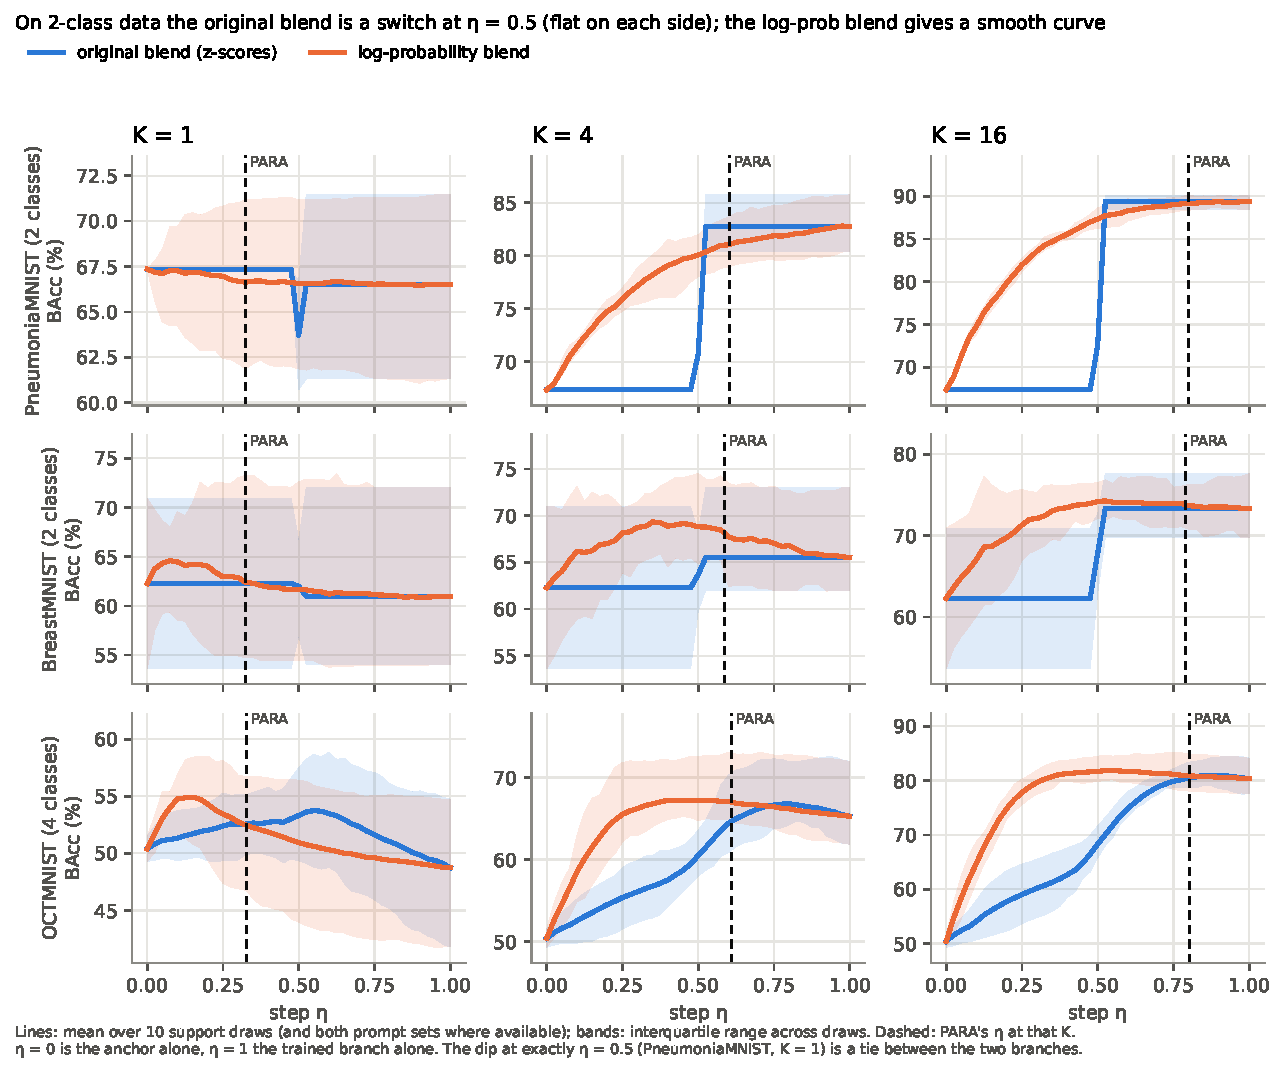
\includegraphics[width=\linewidth]{F3_eta_curves}
  \caption{BAcc as a function of the step $\eta$ for the standardized blend of Eq.~\eqref{eq:blend} (blue) and the log-probability blend of
  Section~\ref{sec:finding4} (orange), on two binary datasets and OCTMNIST.
  Lines: mean over 10 support draws and the available prompt sets; bands: interquartile range over draws.
  Dashed: PARA's step at that $K$. $\eta = 0$ is the anchor alone and $\eta = 1$ the trained branch alone.
  On the binary datasets the standardized blend is flat on each side of $\eta = 0.5$; the dip at exactly $\eta = 0.5$
  (PneumoniaMNIST, $K = 1$) is a tie between disagreeing branches.}
  \label{fig:eta_curves}
\end{figure}

\begin{table}[t]
\centering
\small
\caption{Mean BAcc (\%) over 10 support draws, averaged over prompt sets. ZS: zero-shot; z: standardized blend; lp: log-probability blend; Shot: shot-only step. Bold: best non-oracle method per row. *Oracle picks $\eta$ on the test set per draw and is not achievable.}
\label{tab:T2a_mean_bacc}
\begin{adjustbox}{max width=\linewidth}
\begin{tabular}{lrrrrrrr}
\toprule
Dataset & $K$ & ZS & Visual & PARA (z) & PARA (lp) & Shot (z) & Oracle (lp)* \\
\midrule
DermaMNIST & 1 & 21.16 & 29.70 & 26.45 & \textbf{29.91} & 28.76 & 32.24 \\
DermaMNIST & 4 & 21.16 & 45.66 & 43.98 & \textbf{46.82} & 46.09 & 47.72 \\
DermaMNIST & 16 & 21.16 & 57.68 & 57.41 & \textbf{57.94} & 57.75 & 58.62 \\
OCTMNIST & 1 & 50.40 & 48.76 & 52.56 & 52.40 & \textbf{52.72} & 56.66 \\
OCTMNIST & 4 & 50.40 & 65.28 & 64.66 & \textbf{66.98} & 66.40 & 68.72 \\
OCTMNIST & 16 & 50.40 & 80.36 & 80.49 & 80.86 & \textbf{80.97} & 82.39 \\
BloodMNIST & 1 & 14.18 & \textbf{57.76} & 34.28 & 53.09 & 43.53 & 58.12 \\
BloodMNIST & 4 & 14.18 & \textbf{82.78} & 69.39 & 81.63 & 75.80 & 82.97 \\
BloodMNIST & 16 & 14.18 & \textbf{90.73} & 88.65 & 90.57 & 89.68 & 90.81 \\
BreastMNIST & 1 & 62.28 & 60.96 & 62.28 & \textbf{62.44} & 62.28 & 70.36 \\
BreastMNIST & 4 & 62.28 & 65.50 & 65.50 & \textbf{67.81} & 65.50 & 73.17 \\
BreastMNIST & 16 & 62.28 & 73.34 & 73.34 & \textbf{73.81} & 73.34 & 76.98 \\
PneumoniaMNIST & 1 & \textbf{67.35} & 66.51 & \textbf{67.35} & 66.59 & \textbf{67.35} & 71.53 \\
PneumoniaMNIST & 4 & 67.35 & \textbf{82.75} & \textbf{82.75} & 81.03 & \textbf{82.75} & 83.41 \\
PneumoniaMNIST & 16 & 67.35 & \textbf{89.40} & \textbf{89.40} & 89.21 & \textbf{89.40} & 89.79 \\
OrganAMNIST & 1 & 25.71 & \textbf{48.97} & 37.30 & 46.79 & 41.52 & 49.59 \\
OrganAMNIST & 4 & 25.71 & \textbf{65.75} & 57.40 & 63.61 & 62.14 & 65.86 \\
OrganAMNIST & 16 & 25.71 & \textbf{81.48} & 79.74 & \textbf{81.48} & 80.59 & 81.71 \\
\bottomrule
\end{tabular}
\end{adjustbox}
\end{table}


\paragraph{Consequences for PARA.}
Because PARA's step is a fixed curve in $K$ (Section~\ref{sec:finding1}), the switch is set by the shot count alone.
On the binary datasets PARA's step never exceeds $0.347$ at $K = 1$ and is never below $0.580$ at $K = 4$,
so PARA \emph{is} zero-shot at $K = 1$ and \emph{is} visual only at $K = 4$ and $16$, on every draw
(Table~\ref{tab:T2a_mean_bacc}: on BreastMNIST, $62.28$ BAcc at $K = 1$, equal to zero-shot, and $65.50$ and $73.34$ at $K = 4$ and $16$, equal to visual only).
The shot-only schedule falls on the same side of $0.5$ at every $K$, which is why the two give identical predictions on the binary datasets in Section~\ref{sec:finding1}.

Two things follow.
First, the worst-case protection that the anchor provides is all or nothing, and which one a user gets depends only on $K$.
At $K = 1$ the switch happens to keep the anchor, which protects the worst draws:
CVaR20 is $67.35$ on PneumoniaMNIST and $62.28$ on BreastMNIST, against $53.21$ and $46.49$ for visual only.
At $K = 4$ on BreastMNIST it drops the anchor entirely: CVaR20 falls to $50.56$, the visual-only value, well below the anchor's $62.28$.
Second, no intermediate step can help, because there is no intermediate prediction.
Even the oracle can only choose a side per draw: its gains (\eg $67.65$ against $62.28$ on BreastMNIST at $K = 1$) come from picking zero-shot on some draws and visual only on others,
not from blending.
A blend that keeps each branch's confidence avoids this; Section~\ref{sec:finding4} evaluates one.

\section{What the step should depend on: the anchor's reliability relative to the trained branch}\label{sec:finding3}

Sections~\ref{sec:finding1} and~\ref{sec:finding2} show that PARA's step depends on $K$ and nothing else.
This section asks what a good step would depend on.
The answer is not the anchor's quality alone but how good the anchor is compared with the branch trained on the support set.
A rule built on the anchor's quality alone, fixed in advance on the design datasets, improved on them and failed on the held-out datasets.

\paragraph{Anchoring helps or hurts depending on the dataset.}
At $K = 1$, where the anchor matters most, it can be either a safeguard or a burden (Figure~\ref{fig:worst_case}).
On OCTMNIST, PneumoniaMNIST and BreastMNIST, where the anchor is about as accurate as the trained branch,
PARA's worst draws are much better than those of the trained branch alone:
CVaR20 is $47.70$ against $37.05$, $67.35$ against $53.21$, and $62.28$ against $46.49$.
On OrganAMNIST and BloodMNIST, where the trained branch is far more accurate, anchoring costs worst-case accuracy:
$34.62$ against $45.34$, and $27.01$ against $50.71$.
PARA's step is the same in all five cases.

\begin{figure}[t]
  \centering
  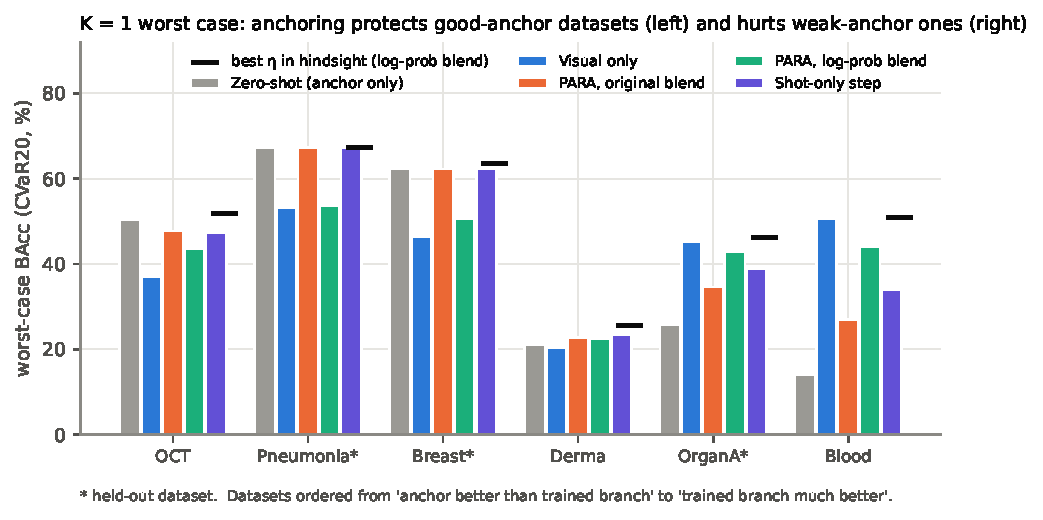
\includegraphics[width=\linewidth]{F5_worst_case_K1}
  \caption{Worst-case BAcc (CVaR20) at $K = 1$.
  The first three datasets are those where the anchor matches or beats the trained branch on mean BAcc at $K = 1$,
  the last three those where the trained branch is better. Held-out datasets are marked with an asterisk.
  The log-probability bars are discussed in Section~\ref{sec:finding4}.}
  \label{fig:worst_case}
\end{figure}

\paragraph{The best step follows relative anchor quality.}
The best step in hindsight (chosen on the test set) varies widely: from $0.17$ to $0.95$ for the log-probability blend of Section~\ref{sec:finding4},
and from $0.49$ to $0.98$ for the standardized blend on the multi-class datasets
(on binary datasets the standardized blend has no unique best step, Section~\ref{sec:finding2}).
It is ordered by the gap between zero-shot and visual-only BAcc (Figure~\ref{fig:best_eta}):
the Spearman correlation is $-0.80$ over all 18 (dataset, $K$) cells for the log-probability blend
and $-0.94$ over the 12 multi-class cells for the standardized blend (both $p < 0.001$).
This gap is computed on test labels, so it is a diagnostic of what the step should track, not a usable rule.
PARA's step, by contrast, is one value per $K$ (the dashed lines).

\begin{figure}[t]
  \centering
  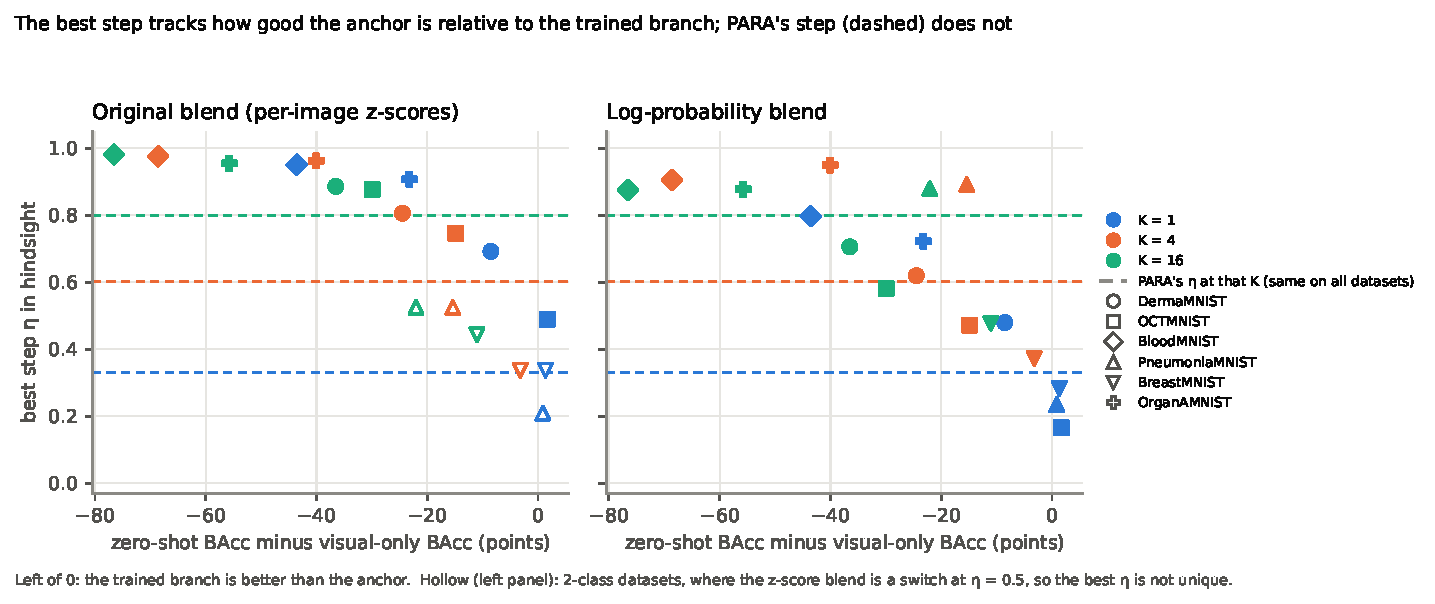
\includegraphics[width=\linewidth]{F4_best_eta_vs_relative_anchor}
  \caption{Best step in hindsight against zero-shot minus visual-only BAcc, one point per dataset and $K$,
  for the standardized blend (left) and the log-probability blend (right).
  Dashed lines: PARA's step at each $K$, which is the same on every dataset.
  Hollow markers (left): binary datasets, where the standardized blend is a switch and the best step is not unique.}
  \label{fig:best_eta}
\end{figure}

\paragraph{A rule fixed in advance: anchor reliability alone.}
A usable rule must estimate reliability from the support set.
The anchor's side is easy to measure, because the anchor is the frozen model:
$r_a$ is the anchor's mean probability for the true class on the support images, rescaled so that chance is $0$ and perfect is $1$.
On the design datasets $r_a$ tracks the best step well (Spearman $-0.71$ over 18 settings, $p < 0.001$).
We therefore fixed, before running any held-out dataset, an \emph{anchor-aware} step that treats the anchor as $k_0$ extra labelled examples:
\begin{equation}
  \eta_{\text{aa}} = \frac{K}{K + k_0}, \qquad k_0 = c\,\frac{r_a}{1 - r_a}, \qquad c = 8,
\end{equation}
so that a useless anchor ($r_a \approx 0$) gives $\eta_{\text{aa}} \approx 1$, and a reliable one keeps the step low until $K$ is large
(the choice of $c$ is described in Section~\ref{sec:setup}).

\paragraph{It worked in-sample and failed on held-out data.}
Table~\ref{tab:T4_preregistered_rule} reports the rule minus each baseline.
On the design datasets it beats PARA by $4.77$ BAcc points (significantly better in 10 of 18 settings, 7 after Holm's correction, worse in none)
and shot-only by $2.12$; choosing $c$ by leave-one-dataset-out instead gives a similar $4.94$ over PARA.
On the held-out datasets it is worse than every baseline:
$-0.68$ BAcc against PARA, $-1.50$ against shot-only and $-2.20$ against visual only,
and its worst case is worse still, with CVaR20 lower by $4.05$, $4.82$ and $1.89$ points.
Against visual only it is significantly worse in 3 of 12 settings (2 after Holm's correction) and better in none.

\begin{table}[t]
\centering
\small
\caption{Anchor-aware rule minus each baseline. Wilcoxon per setting over 10 draws; counts of settings significantly better/worse ($p<0.05$). ``Holm'' applies Holm's correction across the settings of each row. With 10 draws the smallest attainable two-sided Wilcoxon $p$ is $2/1024 \approx 0.002$, so a Holm-significant setting is one where nearly every draw moves the same way. LODO picks $c$ by mean BAcc on the other design datasets. Counts of draws won and lost are in the CSV.}
\label{tab:T4_preregistered_rule}
\begin{adjustbox}{max width=\linewidth}
\begin{tabular}{llrrllrllr}
\toprule
Setting & vs & $n$ & $\Delta$BAcc & sig. & Holm & $\Delta$F1 & sig. (F1) & Holm (F1) & $\Delta$CVaR20 \\
\midrule
Design, in-sample (frozen c=8) & PARA & 18 & 4.77 & 10/0 & 7/0 & 5.00 & 9/2 & 7/1 & 4.05 \\
Design, in-sample (frozen c=8) & Shot-only & 18 & 2.12 & 6/0 & 6/0 & 2.17 & 7/3 & 6/2 & 2.21 \\
Design, in-sample (frozen c=8) & Visual only & 18 & 0.23 & 2/1 & 0/0 & 0.00 & 3/1 & 1/0 & 1.84 \\
Design, leave-one-dataset-out & PARA & 18 & 4.94 & 10/0 & 6/0 & 5.51 & 9/3 & 6/1 & 3.23 \\
Design, leave-one-dataset-out & Shot-only & 18 & 2.29 & 6/0 & 6/0 & 2.67 & 6/4 & 6/2 & 1.39 \\
Design, leave-one-dataset-out & Visual only & 18 & 0.40 & 3/1 & 1/0 & 0.51 & 4/2 & 0/0 & 1.02 \\
Held-out (frozen c=8) & PARA & 12 & -0.68 & 1/1 & 1/0 & -0.26 & 3/1 & 1/0 & -4.05 \\
Held-out (frozen c=8) & Shot-only & 12 & -1.50 & 1/3 & 1/1 & -1.16 & 2/2 & 1/1 & -4.82 \\
Held-out (frozen c=8) & Visual only & 12 & -2.20 & 0/3 & 0/2 & -3.08 & 0/4 & 0/3 & -1.89 \\
\bottomrule
\end{tabular}
\end{adjustbox}
\end{table}


\paragraph{Why it failed.}
Each held-out dataset broke the rule in a different way, and all three point to the missing half of the comparison.
\begin{itemize}
  \item \emph{OrganAMNIST: a decent anchor, a much better trained branch.}
  Its anchor reliability ($r_a = 0.196$) is higher than OCTMNIST's ($0.164$), so the rule keeps the step low ($0.367$ at $K = 1$).
  But the trained branch is far ahead (visual only $48.97$ BAcc against $25.71$ for zero-shot), and the best step is $0.91$.
  The rule reaches $37.86$; visual only reaches $48.97$.
  Over all 21 multi-class settings, including OrganAMNIST, the correlation between $r_a$ and the best step drops to $-0.45$.
  \item \emph{PneumoniaMNIST at $K = 4$: the anchor is good, but not good enough.}
  Its high anchor reliability (mean $r_a = 0.392$) keeps the step below the binary switch point on 7 of 10 draws (mean step $0.415$),
  so on those draws the rule returns the anchor. It reaches $71.12$ BAcc, while the trained branch has already reached $82.75$.
  \item \emph{BreastMNIST at $K = 1$: an unstable estimate.}
  With one image per class, $r_a$ varies so much between draws that the step falls on either side of the switch point
  (above $0.5$ on 11 of 20 draws, mean $0.528$).
  The draws that switch to the trained branch include its worst ones:
  CVaR20 is $46.49$, the visual-only value, against $62.28$ for PARA, which always stayed with the anchor.
\end{itemize}
In each case the rule saw only the anchor's reliability, while the right step depends on the anchor relative to a trained branch it cannot see.
The trained branch's reliability is hard to estimate on the support set, because the branch is fitted to those same images;
a reliability estimated in the frozen space underestimates the trained branch, and the step we built from it was worse than PARA's
($54.73$ against $57.54$ mean BAcc on the design datasets; Appendix~B).

\paragraph{Measuring the trained branch directly.}
The HOSO-style step does measure the trained branch, by holding out one shot per class.
Where the support set is large enough it can be accurate: on OrganAMNIST it comes within $0.10$ and $0.16$ points of the oracle at $K = 4$ and $16$
($65.75$ against $65.85$, $81.46$ against $81.62$).
On the binary datasets, a single held-out image per class makes it noisy:
on PneumoniaMNIST at $K = 16$ it reaches $83.31$ BAcc against $89.40$ for PARA, and its worst case falls back to the anchor's $67.35$ against $87.22$.
It also needs an extra training run per draw and cannot be used at $K = 1$.
A cheap, reliable estimate of the trained branch's accuracy relative to the anchor is, in our view, the missing ingredient for an adaptive step.

\section{The blend space matters: a log-probability blend}\label{sec:finding4}

Section~\ref{sec:finding2} traced the binary switch to the standardization in Eq.~\eqref{eq:blend}, which discards each branch's confidence.
A natural correction is to blend the branches' log-probabilities instead, keeping PARA's step unchanged:
\begin{equation}
  \hat z(x) = (1 - \eta)\,\log \operatorname{softmax}\big(z^0(x)\big) + \eta\,\log \operatorname{softmax}\big(z^S(x)\big).
  \label{eq:logprob}
\end{equation}
Each branch keeps its own temperature ($\tau_0$ for the anchor, the learned $\tau_v$ for the support branch),
so a confident branch can outweigh an unsure one, also with two classes.
Eq.~\eqref{eq:logprob} adds no parameter and uses the same step values and the same trained models as before;
only the way the two predictions are combined changes.
We were led to it by the binary failure seen on the held-out datasets, so we present it as a principled correction to be tested further,
not as a new method.
Because nothing in it is fitted, we evaluate it on all six datasets.

\paragraph{Same step, better predictions on multi-class tasks.}
At PARA's own step, the log-probability blend improves mean BAcc by $4.86$ points on the multi-class datasets
(Table~\ref{tab:T3_paired_tests}; significantly better in 14 of 21 settings, 10 after Holm's correction, worse in none)
and Macro-F1 by $5.67$.
The gains are largest where the anchor is weakest and PARA's step keeps too much of it.
On BloodMNIST at $K = 1$, mean BAcc rises from $34.28$ to $53.09$ and CVaR20 from $27.01$ to $43.96$;
on OrganAMNIST at $K = 1$, CVaR20 rises from $34.62$ to $43.00$ (Table~\ref{tab:T2b_cvar20_bacc}).
On the binary datasets the mean gain is small ($0.36$ BAcc; 2 of 9 settings better, 1 after Holm's correction, none worse),
and all of it comes from BreastMNIST; on PneumoniaMNIST the log-probability blend is slightly worse at every $K$.

\begin{table}[t]
\centering
\small
\caption{Paired differences over support draws. Wilcoxon signed-rank per (dataset, prompt set, K) setting; counts of settings significantly better/worse at $p<0.05$. ``Holm'' applies Holm's correction across the settings of each row. With 10 draws the smallest attainable two-sided Wilcoxon $p$ is $2/1024 \approx 0.002$, so a Holm-significant setting is one where nearly every draw moves the same way. $\Delta$CVaR20 is the mean over settings. (b) uses PARA's step for both blends. Counts of draws won and lost are in the CSV.}
\label{tab:T3_paired_tests}
\begin{adjustbox}{max width=\linewidth}
\begin{tabular}{llrrllrllr}
\toprule
Comparison & Group & $n$ & $\Delta$BAcc & sig. & Holm & $\Delta$F1 & sig. (F1) & Holm (F1) & $\Delta$CVaR20 \\
\midrule
(a) shot-only minus PARA & binary & 9 & 0.00 & 0/0 & 0/0 & 0.00 & 0/0 & 0/0 & 0.00 \\
(a) shot-only minus PARA & multi-class & 21 & 2.74 & 16/0 & 11/0 & 2.95 & 15/1 & 10/0 & 2.01 \\
(a) shot-only minus PARA & design & 18 & 2.65 & 13/0 & 8/0 & 2.84 & 12/1 & 7/0 & 1.84 \\
(a) shot-only minus PARA & held-out & 12 & 0.82 & 3/0 & 3/0 & 0.90 & 3/0 & 3/0 & 0.76 \\
(b) log-prob minus z-score & binary & 9 & 0.36 & 2/0 & 1/0 & 1.00 & 2/2 & 2/0 & -2.67 \\
(b) log-prob minus z-score & multi-class & 21 & 4.86 & 14/0 & 10/0 & 5.67 & 13/1 & 9/0 & 3.12 \\
\bottomrule
\end{tabular}
\end{adjustbox}
\end{table}


\paragraph{The cost: worst-case protection where the anchor is good.}
The same property that helps weak anchors hurts good ones.
At $K = 1$ on the three datasets where the anchor matches the trained branch, CVaR20 falls:
from $67.35$ to $53.59$ on PneumoniaMNIST, from $62.28$ to $50.55$ on BreastMNIST, and from $47.70$ to $43.50$ on OCTMNIST
(Figure~\ref{fig:worst_case}, green bars).
On the binary datasets the worst case falls by $2.67$ points on average over settings.
On the two binary datasets, PARA at $K = 1$ under the standardized blend returned the anchor on every image and so inherited its stable worst case.
Under the log-probability blend the support branch can overrule the anchor wherever it is more confident,
including on the poor draws where its confident predictions are wrong.
We did not measure calibration directly; this explanation is consistent with the pattern but remains a hypothesis.
\begin{table}[t]
\centering
\small
\caption{CVaR20 BAcc (\%): mean of the worst 2 of 10 support draws, averaged over prompt sets. Bold: best non-oracle method per row. *Oracle picks $\eta$ on the test set per draw and is not achievable.}
\label{tab:T2b_cvar20_bacc}
\begin{tabular}{lrrrrrrr}
\toprule
Dataset & K & Zero-shot & Visual only & PARA (z) & PARA (log-prob) & Shot-only (z) & Oracle (log-prob)* \\
\midrule
DermaMNIST & 1 & 21.16 & 20.41 & 22.70 & 22.40 & \textbf{23.33} & 25.63 \\
DermaMNIST & 4 & 21.16 & 39.41 & 39.04 & 40.27 & \textbf{40.87} & 41.71 \\
DermaMNIST & 16 & 21.16 & 54.62 & 54.20 & 54.77 & \textbf{54.90} & 55.34 \\
OCTMNIST & 1 & \textbf{50.40} & 37.05 & 47.70 & 43.50 & 47.28 & 51.93 \\
OCTMNIST & 4 & 50.40 & 46.77 & \textbf{52.60} & 49.60 & 50.55 & 55.23 \\
OCTMNIST & 16 & 50.40 & 71.92 & 73.58 & 72.95 & \textbf{73.65} & 75.23 \\
BloodMNIST & 1 & 14.18 & \textbf{50.71} & 27.01 & 43.96 & 33.97 & 50.83 \\
BloodMNIST & 4 & 14.18 & \textbf{77.85} & 64.64 & 76.66 & 72.11 & 78.00 \\
BloodMNIST & 16 & 14.18 & \textbf{89.28} & 86.71 & 89.04 & 88.10 & 89.38 \\
BreastMNIST & 1 & \textbf{62.28} & 46.49 & \textbf{62.28} & 50.55 & \textbf{62.28} & 63.47 \\
BreastMNIST & 4 & \textbf{62.28} & 50.56 & 50.56 & 57.17 & 50.56 & 68.17 \\
BreastMNIST & 16 & 62.28 & 66.84 & 66.84 & \textbf{67.12} & 66.84 & 72.21 \\
PneumoniaMNIST & 1 & \textbf{67.35} & 53.21 & \textbf{67.35} & 53.59 & \textbf{67.35} & 67.35 \\
PneumoniaMNIST & 4 & 67.35 & \textbf{76.32} & \textbf{76.32} & 75.94 & \textbf{76.32} & 76.84 \\
PneumoniaMNIST & 16 & 67.35 & \textbf{87.22} & \textbf{87.22} & 86.99 & \textbf{87.22} & 87.46 \\
OrganAMNIST & 1 & 25.71 & \textbf{45.34} & 34.62 & 43.00 & 38.97 & 46.12 \\
OrganAMNIST & 4 & 25.71 & \textbf{59.99} & 53.06 & 58.25 & 56.71 & 60.02 \\
OrganAMNIST & 16 & 25.71 & \textbf{80.32} & 78.19 & 80.29 & 79.35 & 80.45 \\
\bottomrule
\end{tabular}
\end{table}


\paragraph{The blend has a real interior, but PARA's step does not fit it.}
Sweeping $\eta$ shows what the log-probability blend makes possible (Figure~\ref{fig:eta_curves}, orange).
The optima below are chosen in hindsight on the mean curve, so they show what a good step could achieve, not what any rule achieved.
On BreastMNIST the curve has an interior optimum that beats both branches, which the standardized blend cannot produce:
$64.60$ BAcc at $\eta = 0.075$ for $K = 1$, $69.33$ at $0.35$ for $K = 4$, and $74.28$ at $0.525$ for $K = 16$,
against best standardized values of $62.28$, $65.50$ and $73.34$.
On PneumoniaMNIST there is no meaningful gain: the best value is the anchor at $K = 1$ and the trained branch at $K = 16$,
and at $K = 4$ the optimum ($82.81$ at $\eta = 0.975$) is within $0.06$ points of the standardized blend.
On OCTMNIST the gains are modest ($1.18$, $0.41$ and $0.91$ points at $K = 1$, $4$ and $16$),
but the optimum sits much lower for the log-probability blend ($0.15$, $0.40$ and $0.55$) than for the standardized one ($0.55$, $0.80$ and $0.875$).
The same $\eta$ therefore means different things in the two blends, and PARA's schedule, calibrated for neither, transfers to neither.
The best step for the log-probability blend still follows relative anchor quality (Figure~\ref{fig:best_eta}, right).

\paragraph{The oracle confirms the direction.}
Choosing the step in hindsight for each draw, the log-probability blend matches or beats the standardized blend in 17 of 18 dataset and $K$ cells
(the exception is DermaMNIST at $K = 16$, by $0.02$ points), with the largest margins on BreastMNIST.
Blending in log-probability space is thus at least as expressive as blending standardized scores, and on binary tasks strictly more so;
what it still needs is a step that knows how reliable each branch is, which is the open problem of Section~\ref{sec:finding3}.

\section{Discussion}\label{sec:discussion}

\paragraph{What PARA's step does, and what a step should do.}
PARA's design rests on two good ideas: keep the frozen prompt prediction as a support-invariant anchor, and move away from it by a step that adapts to the support set.
Our analysis supports the first and not the second, at least in BiomedCLIP's frozen space.
The geometric signals in Eq.~\eqref{eq:eta} mostly measure properties of the pretrained model, the gap between modalities and the narrow cone of image embeddings,
so the step becomes a fixed function of $K$ (Section~\ref{sec:finding1}).
The standardized blend then turns that step into a switch on binary tasks (Section~\ref{sec:finding2}).
Neither observation is a flaw in the idea of anchoring; both concern how the step is computed and applied.
What the step should track is the reliability of the trained branch relative to the anchor (Section~\ref{sec:finding3}),
and the blend should let each branch's confidence count (Section~\ref{sec:finding4}).
Neither is solved here.
The anchor's side of the comparison is easy to estimate on the support set; the trained branch's side is not, because the branch is fitted to those same images.
The log-probability blend helps on multi-class tasks but costs worst-case accuracy where the anchor is good, which suggests that the branches' confidences need calibrating before they are blended.

\paragraph{Recommendations for evaluating adaptive blending.}
Four practices would have exposed these effects early, and we suggest them for future work on prompt-anchored or residual adaptation.
\begin{enumerate}
  \item \emph{Check that an adaptive signal adapts.} Report how much the step varies across support draws and whether it tracks the best step per draw.
  A step with a standard deviation near $0.01$ across draws is a schedule, whatever its formula.
  \item \emph{Compare against the simplest baselines on the same trained models:} zero-shot, visual only, and a step that depends only on $K$.
  Here the shot-only schedule beat the adaptive step, and on binary tasks both reduced to one of the two branches.
  \item \emph{Include binary tasks and balanced metrics.} The switch of Section~\ref{sec:finding2} is invisible on multi-class benchmarks,
  and plain accuracy can reward majority-class predictions (DermaMNIST in our setup).
  \item \emph{Report worst-case alongside mean performance, and test rules on data not used to design them.}
  The anchor-aware rule looked convincing on the design datasets and failed on held-out ones;
  its worst case moved further than its mean.
\end{enumerate}

\paragraph{Scope.}
Our claims concern PARA's step and blend as specified in the paper, reimplemented without official code, and studied in few-shot classification.
PARA also reports base-to-novel generalization \citep{kang2026para}, which we do not examine.
Finding~1 follows from two properties of the frozen space, the modality gap and the narrow image cone, which are known for CLIP-style models generally \citep{liang2022mind};
we expect it to carry over, but we tested only BiomedCLIP.
Finding~2 follows from the standardization alone and holds for any backbone with two classes.

\paragraph{Limitations.}
\begin{itemize}
  \item \emph{One training seed and three shot levels.} Each support draw is trained once, so draw-to-draw variation includes optimization noise.
  We use $K \in \{1, 4, 16\}$ only.
  \item \emph{Datasets and resolution.} We use MedMNIST v2 at $128$ or $224$ pixels with MedMNIST splits and fixed test subsets,
  so absolute numbers are not comparable to the paper's benchmark.
  Three held-out datasets is a small test: two are binary, only OrganAMNIST is multi-class, and BreastMNIST has 156 test images.
  \item \emph{Dependence between settings.} The two prompt sets of a dataset share their support draws, so settings are not independent and pooled counts overstate the evidence;
  the per-setting tests are the safer reading.
  With 10 draws per setting, the smallest attainable Wilcoxon $p$ is about $0.002$, which limits how many settings can survive Holm's correction.
  \item \emph{The anchor-aware constant.} $c = 8$ was chosen in-sample on the design datasets.
  We chose it before training on any held-out dataset, but the choice itself was not recorded with a date (Section~\ref{sec:setup}),
  and leave-one-dataset-out by the same CVaR20 criterion picks a different $c$ for each left-out dataset.
  \item \emph{The log-probability blend was motivated by held-out results.} It has no fitted parameters, but the idea came after we saw the binary failure,
  so its binary results are not a clean held-out test.
  \item \emph{Hindsight quantities.} The oracle step, the best points on the $\eta$ curves, and the zero-shot minus visual-only gap all use test labels.
  We use them only to describe what a good step would do, never as rules.
  \item \emph{Baselines are adapted.} The HOSO-style step chooses PARA's $\eta$ on one held-out shot per class; it follows the idea of \citet{vorster2026hoso}
  but is not their method, which learns the ratio by gradient descent.
\end{itemize}

\paragraph{Future work.}
The most useful next step is an estimate of the trained branch's reliability relative to the anchor that needs no test labels,
for example from held-out shots when $K$ allows, or from agreement between the branches on unlabelled images.
A second is calibrated blending: rescaling each branch's confidence on the support set before combining log-probabilities,
which may keep the multi-class gains of Section~\ref{sec:finding4} without the loss in worst case.
Both should be tested on more held-out datasets, more seeds and a second backbone.

\section{Conclusion}\label{sec:conclusion}
PARA keeps a frozen prompt prediction as an anchor and moves away from it by a step computed from the support set.
In BiomedCLIP, that step is set by the number of shots and not by the support set, because its geometric signals reflect the pretrained space rather than the classes;
on binary tasks the standardized blend turns it into a choice between the anchor and the trained branch.
A schedule in $K$ alone does as well or better.
What the step should depend on is how reliable the anchor is relative to the trained branch; a rule based on the anchor alone did not survive held-out testing,
and blending log-probabilities helps on multi-class tasks at a cost in worst-case accuracy.
Measuring the trained branch's reliability, and calibrating both branches before blending, are the open problems for anchored few-shot adaptation.


\bibliographystyle{plainnat}
\bibliography{refs}
\end{document}
